\section{Introduction}

\begin{description}[font=\quad $\circ$, topsep=-2pt, itemsep=2pt]
	\item Rovers have been widely employed by military and research community (space research) to explore unknown terrains. However rovers have also been in use for simpler applications such as monitoring of different zones on the factory floor. Be it simple or complex rover, they present two major challenges:
	
	\begin{enumerate}[itemsep=0em]
		\item Interaction with the environment
		\item Wireless control
	\end{enumerate}
	
	\item In comparison with the scientific Mars rovers which are voluminous beasts of the order of a few hundred kilograms \cite{RobotSizes}, our rover is a simple three-wheeled bot weighing slightly more than a 1500 grams. The motors power the back wheels and the front wheel is simply a ball-bearing with a low coefficient of friction, allowing the rover to move quickly over smooth surfaces.

	\clearpage
	\quad A block-diagram of the overall hardware system is as follows:

	\begin{figure}[ht]	% Source: http://tex.stackexchange.com/q/131259/110560
		\centering
		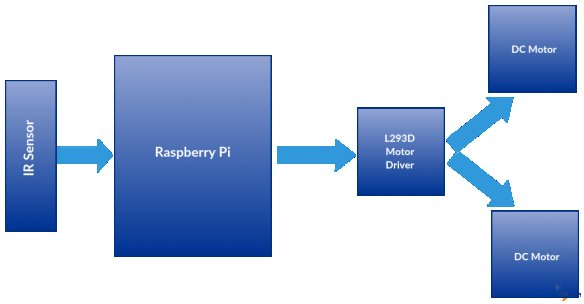
\includegraphics[width=\linewidth]{"./system_diagram.jpg"}
		\caption{System diagram of the rover}
		\label{fig:System Diagram}
	\end{figure}

	\item The microcontroller used is the Raspberry Pi 3, a popular and well-supported hobbyist board. It comes bundled with an onboard Wireless chip and 40 General Purpose Input/Output pins for interfacing with the motors and IR sensors. Power is supplied via a pair of 9v batteries (to the motors) and a 5600 mAh powerbank (to the Pi). The controlling GUI is served by a Python Django server running on Raspbian, a Linux-based distribution installed on the Raspberry Pi’s external memory.

	\item The DC motors that move the rover around are standard 1000 rpm high-torque motors \cite{1000RPMMotors} (low torque motors were unsuccessful in moving the rover on even flat surfaces). The power is delivered via 9v batteries, and controlled via a L293D motor driver. 


	\item An important module of the rover is the trio of IR sensors on the bottom panel, around one inch above the ground. They are used to detect the terrain (black or white) and can be used for line-following even in dim environment. While sufficient for our current purposes, it is possible to replace them with complex, application-specific sensors if required e.g. landmine-detection apparatus for military use cases. \\

	\begin{figure}[ht]	% Source: http://tex.stackexchange.com/q/131259/110560
		\centering
		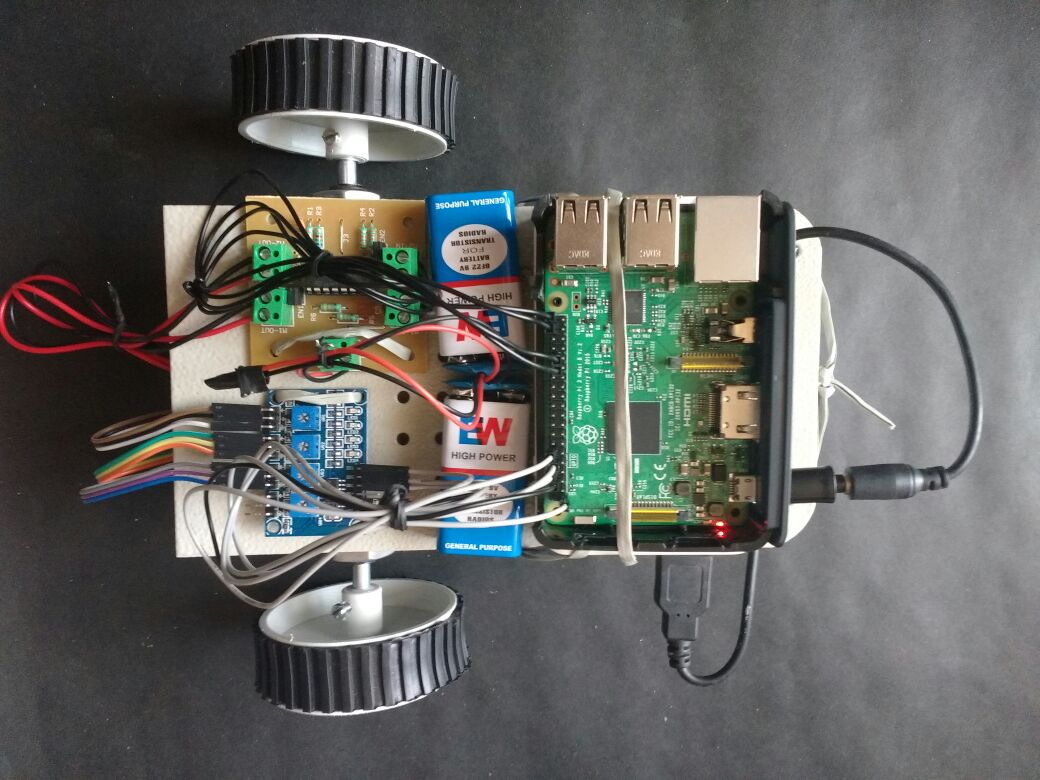
\includegraphics[width=\linewidth]{"./bot-pic-top.jpg"}
		\caption{A photograph of the assembled rover}
		\label{fig:BotPicTop}
	\end{figure}
	
\end{description}

While not nearly state-of-the-art, this setup is sufficient for the proof-of-concept which we build.

